\documentclass[12pt]{article}
\usepackage[english,greek]{babel}
\usepackage[utf8]{inputenc}
\usepackage{nimbusserif}
\usepackage[T1]{fontenc}
\usepackage[margin=1cm,a2paper,landscape]{geometry}
\usepackage{amsmath}
\let\myBbbk\Bbbk
\let\Bbbk\relax
\usepackage[amsbb,subscriptcorrection,zswash,mtpcal,mtphrb,mtpfrak]{mtpro2}
\usepackage{tikz,graphicx,multicol,multirow,enumitem,tabularx,mathimatika,gensymb,venndiagram,hhline,longtable,tkz-euclide,fontawesome5,eurosym,tcolorbox,tabularray}
\usetikzlibrary{3d}
\usetikzlibrary{calc}
\usetikzlibrary{angles}
\tcbuselibrary{skins,theorems,breakable}
\newlist{rlist}{enumerate}{3}
\setlist[rlist]{itemsep=0mm,label=\roman*.}
\newlist{alist}{enumerate}{3}
\setlist[alist]{itemsep=0mm,label=\alph*.}
\newlist{balist}{enumerate}{3}
\setlist[balist]{itemsep=0mm,label=\bf\alph*.}
\newlist{Alist}{enumerate}{3}
\setlist[Alist]{itemsep=0mm,label=\Alph*.}
\newlist{bAlist}{enumerate}{3}
\setlist[bAlist]{itemsep=0mm,label=\bf\Alph*.}
\renewcommand{\textstigma}{\textsigma\texttau}
\newlist{thema}{enumerate}{3}
\setlist[thema]{label=\bf\large{ΘΕΜΑ \textcolor{black}{\Alph*}},itemsep=0mm,leftmargin=0cm,itemindent=18mm}
\newlist{erwthma}{enumerate}{3}
\setlist[erwthma]{label=\bf{\large{\textcolor{black}{\Alph{themai}.\arabic*}}},itemsep=0mm,leftmargin=0.8cm}

\newcommand{\lysh}{\textcolor{black}{\textbf{\faCheck\ \ ΛΥΣΗ}}}
\renewcommand{\textstigma}{\textsigma\texttau}
%----------- ΟΡΙΣΜΟΣ------------------
\newcounter{orismos}[section]
\renewcommand{\theorismos}{\thesection.\arabic{orismos}}   
\newcommand{\Orismos}{\refstepcounter{orismos}{\textbf{\textcolor{black}{\kerkissans{Ορισμός\hspace{2mm}\theorismos}}\;:\;}{}}}

\newenvironment{orismos}[1]
{\begin{tcolorbox}[title=\Orismos {\textcolor{black}{\kerkissans{#1}}},breakable,bottomtitle=-1.5mm,
enhanced standard,titlerule=-.2pt,toprule=0pt, rightrule=0pt, bottomrule=0pt,
colback=white,left=2mm,top=1mm,bottom=0mm,
boxrule=0pt,
colframe=white,borderline west={1.5mm}{0pt}{black},leftrule=2mm,sharp corners,coltitle=black]}
{\end{tcolorbox}}

\newcommand{\kerkissans}[1]{{\fontfamily{maksf}\selectfont \textbf{#1}}}
\renewcommand{\textdexiakeraia}{}

\usepackage[
backend=biber,
style=alphabetic,
sorting=ynt
]{biblatex}
\DeclareTblrTemplate{caption}{nocaptemplate}{}
\DeclareTblrTemplate{capcont}{nocaptemplate}{}
\DeclareTblrTemplate{contfoot}{nocaptemplate}{}
\NewTblrTheme{mytabletheme}{
  \SetTblrTemplate{caption}{nocaptemplate}{}
  \SetTblrTemplate{capcont}{nocaptemplate}{}
  \SetTblrTemplate{contfoot}{nocaptemplate}{}
}

\NewTblrEnviron{mytblr}
\SetTblrStyle{firsthead}{font=\bfseries}
\SetTblrStyle{firstfoot}{fg=red2}
\SetTblrOuter[mytblr]{theme=mytabletheme}
\SetTblrInner[mytblr]{
rowspec={t{7mm}},columns = {c},
  width = 0.85\linewidth,
  row{odd} = {bg=red9,fg=black,ht=8mm},
 row{even} = {bg=red7,fg=black,ht=8mm},
hlines={white},vlines={white},
row{1} = {bg=red4, fg=white, font=\Large\bfseries\fontfamily{maksf}},rowhead = 1,
  hline{2} = {.7mm}, % midrule  
}

\newlist{stoixeia}{itemize}{1}
\setlist[stoixeia]{label=\faCaretRight,noitemsep}


\begin{document}
\begin{mytblr}{rows={m},column{2}={6cm,l}}
Σχήμα & Στοιχεία και τύποι\\
{\kerkissans{Τετράγωνο}\\
\begin{tikzpicture}
\tkzDefPoint(0,2.5){A}
\tkzDefPoint(2.5,2.5){B}
\tkzDefPoint(2.5,0){C}
\tkzDefPoint(0,0){D}
\tkzMarkRightAngle(C,D,A)
\tkzMarkRightAngle(D,A,B)
\tkzMarkRightAngle(A,B,C)
\tkzMarkRightAngle(B,C,D)
\tkzDrawPolygon[plm](A,B,C,D)
\tkzDrawPoints[fill=white](A,B,C,D)
\tkzLabelSegment(B,C){$a$}
\tkzLabelSegment[below](C,D){$a$}
\tkzLabelPoint[left](A){$A$}
\tkzLabelPoint[right](B){$B$}
\tkzLabelPoint[right](C){$\Gamma$}
\tkzLabelPoint[left](D){$\Delta$}
\end{tikzpicture}
} & {\kerkissans{Στοιχεία}\begin{stoixeia}
\item $a$ : Πλευρά
\end{stoixeia}\kerkissans{Τύποι}\begin{itemize}[noitemsep]
\item  $\Pi=4a$
\item  $E=a^2$
\end{itemize}}\\

{\kerkissans{Ορθογώνιο}\\
\begin{tikzpicture}
\tkzDefPoint(0,2){A}
\tkzDefPoint(3,2){B}
\tkzDefPoint(3,0){C}
\tkzDefPoint(0,0){D}
\tkzMarkRightAngle(C,D,A)
\tkzMarkRightAngle(D,A,B)
\tkzMarkRightAngle(A,B,C)
\tkzMarkRightAngle(B,C,D)
\tkzDrawPolygon[plm](A,B,C,D)
\tkzDrawPoints[fill=white](A,B,C,D)
\tkzLabelSegment(B,C){$\pi$}
\tkzLabelSegment[below](C,D){$\mu$}
\tkzLabelPoint[left](A){$A$}
\tkzLabelPoint[right](B){$B$}
\tkzLabelPoint[right](C){$\Gamma$}
\tkzLabelPoint[left](D){$\Delta$}
\end{tikzpicture}
} & {\kerkissans{Στοιχεία}\begin{stoixeia}
\item $\mu$ : Μήκος
\item $\pi$ : Πλάτος
\end{stoixeia}\kerkissans{Τύποι}\begin{itemize}[noitemsep]
\item  $\Pi=2\mu+2\pi$
\item  $E=\mu \pi$
\end{itemize}}\\

{\kerkissans{Παραλληλόγραμμο}\\
\begin{tikzpicture}
\tkzDefPoint(1,2){A}
\tkzDefPoint(4,2){B}
\tkzDefPoint(3,0){C}
\tkzDefPoint(0,0){D}
\tkzDefPoint(1,0){K}
\tkzDefPointBy[projection=onto B--C](A)
\tkzGetPoint{L}
\tkzMarkRightAngle(C,K,A)
\tkzMarkRightAngle(B,L,A)
\tkzDrawPolygon[plm](A,B,C,D)
\tkzDrawSegment[pl](A,K)
\tkzDrawSegment[pl](A,L)
\tkzDrawPoints[fill=white](A,B,C,D)
\tkzLabelSegment[below](C,D){$a$}
\tkzLabelSegment(B,C){$\beta$}
\tkzLabelSegment[yshift=-2mm](A,L){$\upsilon_{\beta}$}
\tkzLabelSegment(A,K){$\upsilon_a$}
\tkzLabelPoint[left](A){$A$}
\tkzLabelPoint[right](B){$B$}
\tkzLabelPoint[right](C){$\Gamma$}
\tkzLabelPoint[left](D){$\Delta$}
\end{tikzpicture}
} & {\kerkissans{Στοιχεία}\begin{stoixeia}
\item $a,\beta$ : Βάσεις (πλευρές)
\item $\upsilon_a,\upsilon_{\beta}$ : Ύψη
\end{stoixeia}\kerkissans{Τύποι}\begin{itemize}[noitemsep]
\item  $\Pi=2a+2\beta$
\item  $E=a \upsilon_a=\beta \upsilon_{\beta}$
\end{itemize}}\\

{\kerkissans{Τρίγωνο}\\
\begin{tikzpicture}
\tkzDefPoint(1,2.5){A}
\tkzDefPoint(0,0){B}
\tkzDefPoint(3.5,0){C}
\tkzDefPoint(1,0){K}
\tkzDefPointBy[projection=onto A--C](B)
\tkzGetPoint{L}
\tkzDefPointBy[projection=onto A--B](C)
\tkzGetPoint{M}
\tkzDrawPolygon[plm](A,B,C)
\tkzDrawSegments[pl](A,K B,L C,M)
\tkzMarkRightAngle(C,K,A)
\tkzMarkRightAngle(B,L,C)
\tkzMarkRightAngle(B,M,C)
\tkzDrawPoints[fill=white](A,B,C)
\tkzLabelSegment(A,C){$\beta$}
\tkzLabelSegment[left](A,B){$\gamma$}
\tkzLabelSegment[below](B,C){$a$}
\tkzLabelSegment[yshift=-8mm](A,K){$\upsilon_a$}
\tkzLabelSegment[right=3mm,yshift=2mm](B,L){$\upsilon_{\beta}$}
\tkzLabelSegment[right](C,M){$\upsilon_{\gamma}$}
\tkzLabelPoint[above](A){$A$}
\tkzLabelPoint[left](B){$B$}
\tkzLabelPoint[right](C){$\Gamma$}
\end{tikzpicture}
} & {\kerkissans{Στοιχεία}\begin{stoixeia}
\item $a,\beta,\gamma$ : Βάσεις (πλευρές)
\item $\upsilon_a,\upsilon_{\beta},\upsilon_{\gamma}$ : Ύψη
\end{stoixeia}\kerkissans{Τύποι}\begin{itemize}[noitemsep]
\item  $\Pi=a+\beta+\gamma$
\item  $E=\dfrac{a\upsilon_a}{2}=\dfrac{\beta\upsilon_{\beta}}{2}=\dfrac{\gamma\upsilon_{\gamma}}{2}$
\end{itemize}}\\

{\kerkissans{Ορθογώνιο τρίγωνο}\\
\begin{tikzpicture}
\tkzDefPoint(0,2.5){B}
\tkzDefPoint(0,0){A}
\tkzDefPoint(3.5,0){C}
\tkzDefPointBy[projection=onto B--C](A)
\tkzGetPoint{K}
\tkzDrawPolygon[plm](A,B,C)
\tkzDrawSegment[pl](A,K)
\tkzMarkRightAngle(C,A,B)
\tkzMarkRightAngle(A,K,C)
\tkzDrawPoints[fill=white](A,B,C)
\tkzLabelSegment[below](A,C){$\beta$}
\tkzLabelSegment[left](A,B){$\gamma$}
\tkzLabelSegment[above](B,C){$a$}
\tkzLabelSegment[below right](A,K){$\upsilon_a$}
\tkzLabelPoint[left](A){$A$}
\tkzLabelPoint[left](B){$B$}
\tkzLabelPoint[right](C){$\Gamma$}
\end{tikzpicture}
} & {\kerkissans{Στοιχεία}\begin{stoixeia}
\item $ a $ Υποτείνουσα
\item $\beta,\gamma$ : Κάθετες πλευρές - Ύψη
\end{stoixeia}\kerkissans{Τύποι}\begin{itemize}[noitemsep]
\item  $\Pi=a+\beta+\gamma$
\item  $E=\dfrac{\beta\gamma}{2}=\dfrac{a\upsilon_a}{2}$
\end{itemize}}\\
\end{mytblr}
\begin{mytblr}{rows={m},column{2}={8.5cm,l}}
Σχήμα & Στοιχεία και τύποι\\
{\kerkissans{Τραπέζιο}\\
\begin{tikzpicture}
\tkzDefPoint(1,2){A}
\tkzDefPoint(2.5,2){B}
\tkzDefPoint(4,0){C}
\tkzDefPoint(0,0){D}
\tkzDefPoint(1,0){K}
\tkzDrawPolygon[plm](A,B,C,D)
\tkzDrawSegment[pl](A,K)
\tkzMarkRightAngle(C,K,A)
\tkzDrawPoints[fill=white](A,B,C,D)
\tkzLabelSegment(A,B){$\beta$}
\tkzLabelSegment[below](C,D){$Β$}
\tkzLabelSegment(A,K){$\upsilon$}
\tkzLabelPoint[left](A){$A$}
\tkzLabelPoint[right](B){$B$}
\tkzLabelPoint[right](C){$\Gamma$}
\tkzLabelPoint[left](D){$\Delta$}
\end{tikzpicture}
} & {\kerkissans{Στοιχεία}\begin{stoixeia}
\item $\beta$ : Μικρή βάση
\item $Β$ : Μεγάλη βάση
\item $\upsilon$ : Ύψος
\end{stoixeia}\kerkissans{Τύποι}\begin{itemize}[noitemsep]
\item  $\Pi=A\varDelta+\beta+B+B\varGamma$
\item  $E=\dfrac{(\beta+B)\upsilon}{2}$
\end{itemize}}\\

{\kerkissans{Κύκλος}\\
\begin{tikzpicture}
\tkzDefPoint(0,0){O}
\tkzDefPoint(1.5,0){A}
\tkzDrawCircle[plm](O,A)
\tkzDrawSegment[pl](O,A)
\tkzDrawPoints[fill=white](A,O)
\tkzLabelSegment(A,O){$\rho$}
\tkzLabelPoint[left](O){$O$}
\tkzLabelPoint[right](A){$A$}
\end{tikzpicture}
} & {\kerkissans{Στοιχεία}\begin{stoixeia}
\item $\rho$ : Ακτίνα
\end{stoixeia}\kerkissans{Τύποι}\begin{itemize}[noitemsep]
\item  $\Pi=2\pi\rho$
\item  $E=\pi\rho^2$
\end{itemize}}\\
{\kerkissans{Ισόπλευρο τρίγωνο}\\
\begin{tikzpicture}
\tkzDefPoint(0,0){B}
\tkzDefPoint(3.5,0){C}
\tkzDefTriangle[equilateral](B,C)
\tkzGetPoint{A}
\tkzDrawPolygon[plm](A,B,C)
\tkzDrawPoints[fill=white](A,B,C)
\tkzLabelSegment(A,C){$a$}
\tkzLabelSegment[below](B,C){$a$}
\tkzLabelSegment[left](A,B){$a$}
\end{tikzpicture}
} & {\kerkissans{Στοιχεία}\begin{stoixeia}
\item $a$ : Πλευρά
\end{stoixeia}\kerkissans{Τύποι}\begin{itemize}[noitemsep]
\item  $\Pi=3α$
\item  $E=\dfrac{a^2\sqrt{3}}{4}$
\end{itemize}}\\

{\kerkissans{Ρόμβος}\\
\begin{tikzpicture}
\tkzDefPoints{0/2/A,1.5/0/B,0/-2/C,-1.5/0/D,0/0/O}
\tkzDrawPolygon[plm](A,B,C,D)
\tkzDrawSegments[pl](A,C B,D)
\tkzDrawPoints[fill=white](A,B,C,D)
\tkzLabelSegment(A,B){$a$}
\tkzLabelSegment[left](A,O){$\delta_1$}
\tkzLabelSegment[below](O,D){$\delta_2$}
\tkzMarkRightAngle(B,O,A)
\tkzLabelPoint[above](A){$A$}
\tkzLabelPoint[right](B){$B$}
\tkzLabelPoint[below](C){$\Gamma$}
\tkzLabelPoint[left](D){$\Delta$}
\end{tikzpicture}
} & {\kerkissans{Στοιχεία}\begin{stoixeia}
\item $a$ : Πλευρά
\item $\delta_1,\delta_2$ : Διαγώνιοι
\end{stoixeia}\kerkissans{Τύποι}\begin{itemize}[noitemsep]
\item  $\Pi=4α$
\item  $E=\dfrac{\delta_1\delta_2}{2}$
\end{itemize}}\\

{\kerkissans{Κανονικό εξάγωνο}\\
\begin{tikzpicture}
\tkzDefPoints{0/0/O,1.75/0/A}
\tkzDefPoint(30:1.51){B}
\tkzDefRegPolygon[center,sides=6,name=P](O,A)
\tkzDrawPolygon[plm](P1,P...,P6)
\tkzDrawSegments[pl](O,P1 O,B)
\tkzLabelSegment[right](P1,P2){$\lambda_6$}
\tkzLabelSegment[above left](O,B){$a_6$}
\tkzLabelPoint[right](P1){$\Gamma$}
\tkzLabelPoint[above](P2){$B$}
\tkzLabelPoint[above](P3){$A$}
\tkzLabelPoint[left](P4){$Z$}
\tkzLabelPoint[below](P5){$E$}
\tkzLabelPoint[below](P6){$\Delta$}
\tkzDrawPoints[fill=white](P1,P...,P6,O)
\end{tikzpicture}
} & {\kerkissans{Στοιχεία}\begin{stoixeia}
\item $\lambda_6$ : Πλευρά
\end{stoixeia}\kerkissans{Τύποι}\begin{itemize}[noitemsep]
\item  $\Pi=6\lambda_6$
\item  $E=3\sqrt{3}\lambda_6^2$
\end{itemize}}\\
\end{mytblr}
\begin{mytblr}{rows={m},column{2}={7cm,l}}
Σχήμα & Στοιχεία και τύποι\\
{\kerkissans{Κύβος}\\
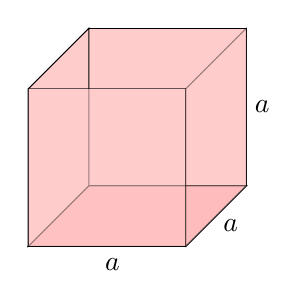
\begin{tikzpicture}
\coordinate (O) at (0,0,0);
\coordinate (A) at (0,2,0);
\coordinate (B) at (0,2,2);
\coordinate (C) at (0,0,2);
\coordinate (D) at (2,0,0);
\coordinate (E) at (2,2,0);
\coordinate (F) at (2,2,2);
\coordinate (G) at (2,0,2);
\draw[fill=red!40] (O) -- (C) -- (G) -- (D) -- cycle;
\draw[fill=red!20,opacity=0.5] (O) -- (C) -- (G) -- (D) -- cycle;
\draw[fill=red!20] (O) -- (A) -- (E) -- (D) -- cycle;
\draw[fill=red!20] (O) -- (A) -- (B) -- (C) -- cycle;
\draw[fill=red!20,opacity=0.4] (D) -- (E) -- (F) -- (G) -- cycle;
\draw[fill=red!20,opacity=0.6] (C) -- (B) -- (F) -- (G) -- cycle;
\tkzText(2.2,1){$a$}
\tkzText(0.3,-1){$a$}
\tkzText(1.8,-.5){$a$}
\end{tikzpicture}
} & {\kerkissans{Στοιχεία}\begin{stoixeia}
\item $a$ : Πλευρά
\end{stoixeia}\kerkissans{Τύποι}\begin{itemize}[noitemsep]
\item  $E=6a^2$
\item  $V=a^3$
\end{itemize}}\\

{\kerkissans{Παραλληλεπίπεδο}\\
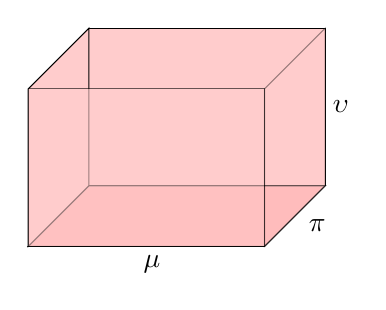
\begin{tikzpicture}
\coordinate (O) at (0,0,0);
\coordinate (A) at (0,2,0);
\coordinate (B) at (0,2,2);
\coordinate (C) at (0,0,2);
\coordinate (D) at (3,0,0);
\coordinate (E) at (3,2,0);
\coordinate (F) at (3,2,2);
\coordinate (G) at (3,0,2);
\draw[fill=red!40] (O) -- (C) -- (G) -- (D) -- cycle;
\draw[fill=red!20,opacity=0.5] (O) -- (C) -- (G) -- (D) -- cycle;
\draw[fill=red!20] (O) -- (A) -- (E) -- (D) -- cycle;
\draw[fill=red!20] (O) -- (A) -- (B) -- (C) -- cycle;
\draw[fill=red!20,opacity=0.4] (D) -- (E) -- (F) -- (G) -- cycle;
\draw[fill=red!20,opacity=0.6] (C) -- (B) -- (F) -- (G) -- cycle;
\tkzText(3.2,1){$\upsilon$}
\tkzText(0.8,-1){$\mu$}
\tkzText(2.9,-.5){$\pi$}
\end{tikzpicture}
} & {\kerkissans{Στοιχεία}\begin{stoixeia}
\item $\mu$ : Μήκος
\item $\pi$ : Πλάτος
\item $\upsilon$ : Ύψος
\end{stoixeia}\kerkissans{Τύποι}\begin{itemize}[noitemsep]
\item  $E=2(\mu\pi+\pi\upsilon+\mu\upsilon)$
\item  $V=\mu\pi\upsilon$
\end{itemize}}\\

{\kerkissans{Σφαίρα}\\
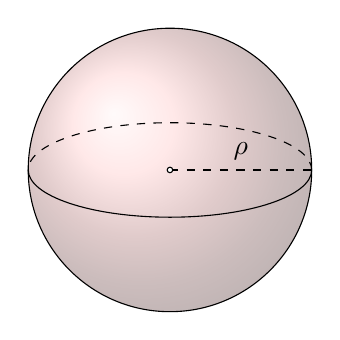
\begin{tikzpicture}
  \shade[ball color = red!30, opacity = 0.4] (0,0) circle (1.8cm);
  \draw (0,0) circle (1.8cm);
  \draw (-1.8,0) arc (180:360:1.8 and 0.6);
  \draw[dashed] (1.8,0) arc (0:180:1.8 and 0.6);
  \draw[dashed] (0,0 ) -- node[above]{$\rho$} (1.8,0);
  \tkzDrawPoint[fill=white](0,0)
\end{tikzpicture}
} & {\kerkissans{Στοιχεία}\begin{stoixeia}
\item $\rho$ : Ακτίνα
\end{stoixeia}\kerkissans{Τύποι}\begin{itemize}[noitemsep]
\item  $E=4\pi\rho^2$
\item  $V=\dfrac{4}{3}\pi\rho^3$
\end{itemize}}\\

{\kerkissans{Κύλινδρος}\\
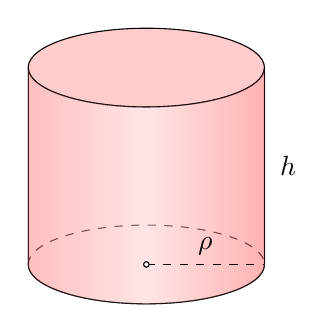
\begin{tikzpicture}
\draw[fill=red!20] (0,0) ellipse (1.5 and 0.5);
\draw (-1.5,0) -- (-1.5,-2.5);
\draw (-1.5,-2.5) arc (180:360:1.5 and 0.5);
\draw [dashed] (-1.5,-2.5) arc (180:360:1.5 and -0.5);
\draw (1.5,-2.5) -- (1.5,0);  
\shadedraw[left color=red!50,
  right color=red!60,
  middle color=red!20,opacity=0.5,shading angle=90] (-1.5,0) -- (-1.5,-2.5) arc (180:360:1.5 and 0.5) -- (1.5,0) arc (0:180:1.5 and -0.5);
\draw[dashed] (0,-2.5) -- node[above]{$\rho$} (1.5,-2.5);
\tkzDrawPoint[fill=white](0,-2.5)
\tkzText(1.8,-1.25){$h$}
\end{tikzpicture}
} & {\kerkissans{Στοιχεία}\begin{stoixeia}
\item $\rho$ : Ακτίνα βάσης
\item $h$ : Ύψος
\end{stoixeia}\kerkissans{Τύποι}\begin{itemize}[noitemsep]
\item  $E=2\pi\rho h+2\pi\rho^2$
\item  $V=\pi\rho^2h$
\end{itemize}}\\

{\kerkissans{Πυραμίδα}\\(Τετράγωνη βάση)\\
\begin{tikzpicture}
\coordinate (O) at (0,0,0);
\coordinate (A) at (-1.2,0,-1.2);
\coordinate (B) at (1.2,0,-1.2);
\coordinate (C) at (1.2,0,1.2);
\coordinate (D) at (-1.2,0,1.2);
\coordinate (K) at (0,2.5,0);
\coordinate (L) at (1.2,0,0);
\draw[plm] (A)--(B)--(C)--(D)--cycle;
\draw[pl,fill=red!30,opacity=0.4] (A)--(B)--(K) -- cycle;
\draw[pl,fill=red!20,opacity=0.4] (A)--(B)--(K) -- cycle;
\draw[pl,fill=red!20,opacity=0.5] (C)--(B)--(K) -- cycle;
\draw[pl,fill=red!20,opacity=0.5] (C)--(D)--(K) -- cycle;
\draw[dashed] (O)--node[right]{$h$}(K) -- node[right]{$s$} (L) -- (O);
\tkzDrawPoint[fill=white](0,0)
\tkzText(-.3,-.7){$a$}
\pic [draw=black, angle radius=0.33cm ] {right angle = C--L--K};
\pic [draw=black, angle radius=0.33cm ] {right angle = L--O--K};
\end{tikzpicture}
} & {\kerkissans{Στοιχεία}\begin{stoixeia}
\item $a$ : Πλευρά βάσης
\item $h$ : Ύψος
\item $s$ : Απόστημα
\end{stoixeia}\kerkissans{Τύποι}\begin{itemize}[noitemsep]
\item  $E=2as+a^2$
\item  $V=\dfrac{1}{3}a^2h$
\end{itemize}}\\

{\kerkissans{Κώνος}\\
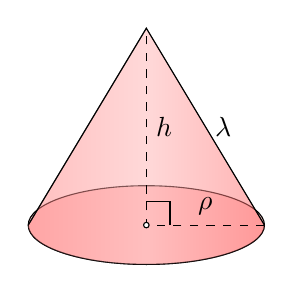
\begin{tikzpicture}
\draw[fill=red!20] (0,0) ellipse (1.5 and 0.5);
\shadedraw[left color=red!50,
  right color=red!60,
  middle color=red!30,opacity=0.5,shading angle=90] (-1.5,0) -- (-0,2.5) -- (1.5,0) arc (180:360:-1.5 and 0.5);
\draw[dashed] (1.5,0) -- node[above]{$\rho$} (0,0)--node[right]{$h$}(0,2.5);
\draw (0.3,0) |- (0,0.3);
\draw (-1.5,0)-- (0,2.5)-- node[right]{$\lambda$} (1.5,0);
\tkzDrawPoint[fill=white](0,0)
\end{tikzpicture}
} & {\kerkissans{Στοιχεία}\begin{stoixeia}
\item $\rho$ : Ακτίνα βάσης
\item $h$ : Ύψος
\item $\lambda$ : Πλευρά
\end{stoixeia}\kerkissans{Τύποι}\begin{itemize}[noitemsep]
\item  $E=\pi\rho\lambda+\pi\rho^2$
\item  $V=\dfrac{1}{3}\pi\rho^2h$
\end{itemize}}\\
\end{mytblr}
\end{document}
